\documentclass[
a4paper, 
12pt, 
]{article}

\usepackage[ngerman,english]{babel}			% Kapitel/Chapter. typographic rules
%\usepackage[english]{babel}
%%%%%%%%%%%%%%
% Format the design


%%%%%%%%%%%%%%%


\usepackage[utf8]{inputenc}			% Encoding with umlauts and ß
%\usepackage{lipsum}				 			% testing text as \lipsum[1-3] 			 
%\usepackage{titling}							% imports \theauthor
\usepackage{graphicx}						% include graphics
\usepackage{siunitx}							% corretct formatting of units
\usepackage[framed,numbered,autolinebreaks,useliterate]{mcode} % for matlab code

\usepackage{amsmath}            % nice equations
\usepackage{url}                			% URLs
%\usepackage{natbib}             		% author-year bibliography style
\usepackage{hyperref}           	% PDF links
%\usepackage{subfig}             	% Subfigures (a), (b), etc
%\usepackage{nomencl}            	% Nomenclature	
\usepackage{tcolorbox}
\usepackage{Systemtheorie}		 	% style with headers/footers/logo/firstpage
\fancyfoot[R]{Juri Fedjaev} 
\usepackage{units}		% nice fractions using \nicefrac

% ----------------------------------------------------------------------------


\begin{document}
	
	\thispagestyle{firstpage} 			% use different style here (from .sty file)
	
	\section*{Neuroprothetik -- Exercise 2: Mathematical Basics I}
	\subsection{Plot slope fields and isocline}
	The following plots show the slope fields for $t \in [-5, 5]s$ and $V \in [-5, 5]V$, and the isocline for (-2, -1, 0, 1, 2)\nicefrac{V}{s} for the following differential equations: 
	\begin{align}
	\frac{dV}{dt} &= 1 - V - t\\
	\frac{dV}{dt} &= sin(t) - \frac{1}{1.5}~V
	\end{align}
\begin{figure}[h]
\centering
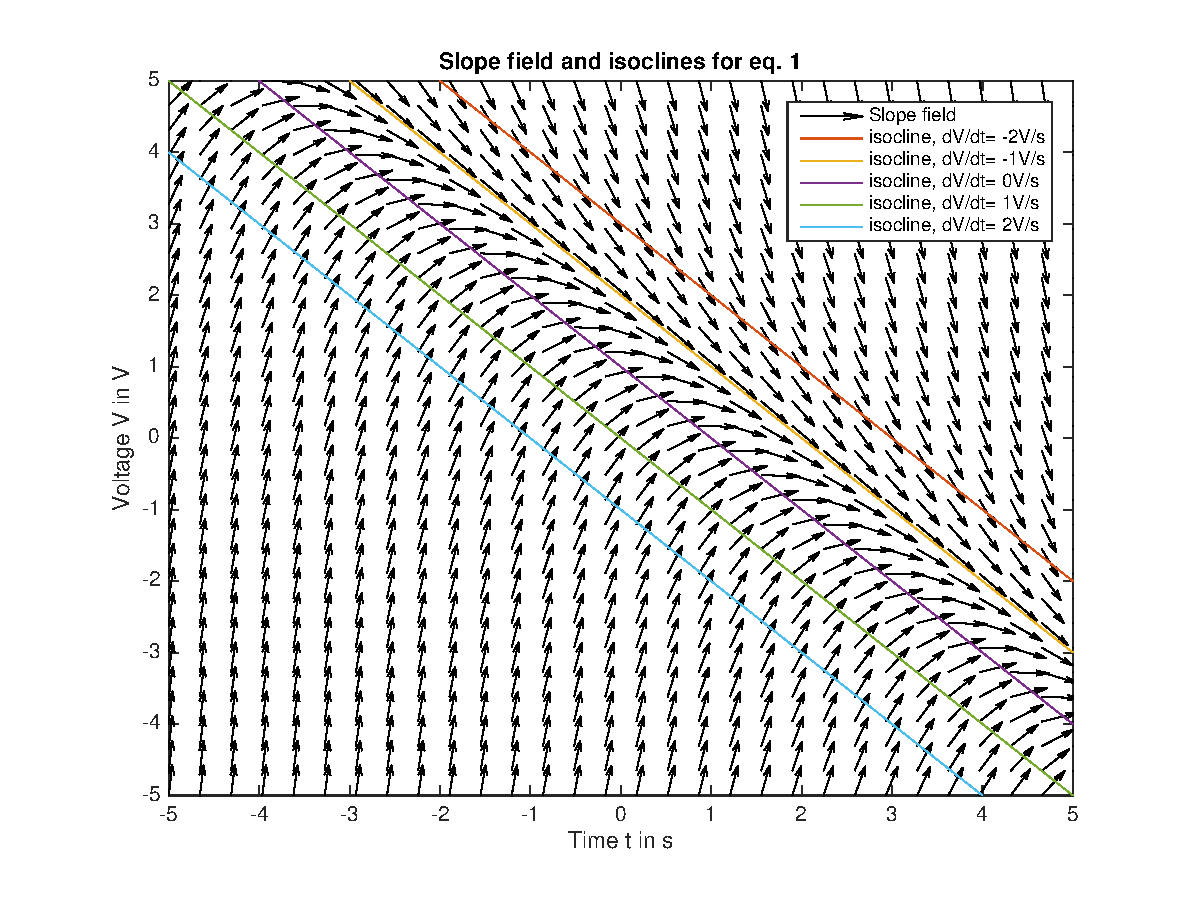
\includegraphics[width=0.85\linewidth]{Plots/eq1_plot}
\caption{Slope field for equation 1 and its corresponding isoclines.}
\label{fig:eq1_plot}
\end{figure}

\begin{figure}[h]
	\centering
	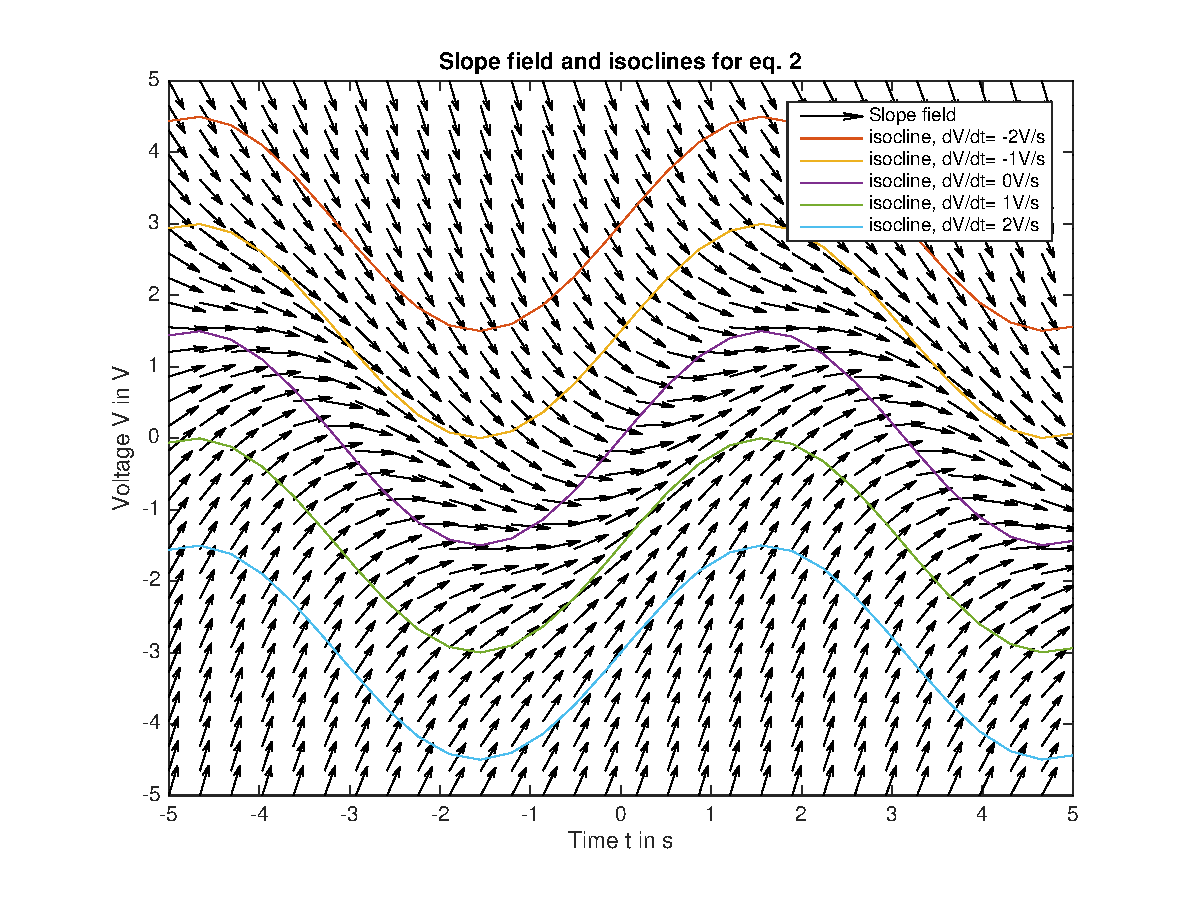
\includegraphics[width=0.85\linewidth]{Plots/eq2_plot}
	\caption{Slope field for equation 2 and its corresponding isoclines.}
	\label{fig:eq2_plot}
\end{figure}

\subsection{Differential equations of a simple cell model}
To derive the differential equation for the equivalent circuit of a leaky integrate and fire neuron, we use Kirchhoff's law: 
\begin{align}
0 &= I_c + I_{R_l} + I_{ex} \\
0 &= C\cdot\frac{du}{dt} + \frac{u}{R_l} + I_{ex} \nonumber \\
\Rightarrow \frac{du}{dt} &= -\frac{1}{C}\left(\frac{u}{R_l} + I_{ex} \right) \nonumber
\end{align}
With $I_{ex} = I_{max}\cdot sin(t)$ this results in:
\begin{align}
\Rightarrow \frac{du}{dt} &= -\frac{1}{C}\left(\frac{u}{R_l} + I_{max}\cdot sin(t) \right) 
\end{align}

\subsubsection*{Plot the slope fields:}
\begin{figure}[h]
\centering
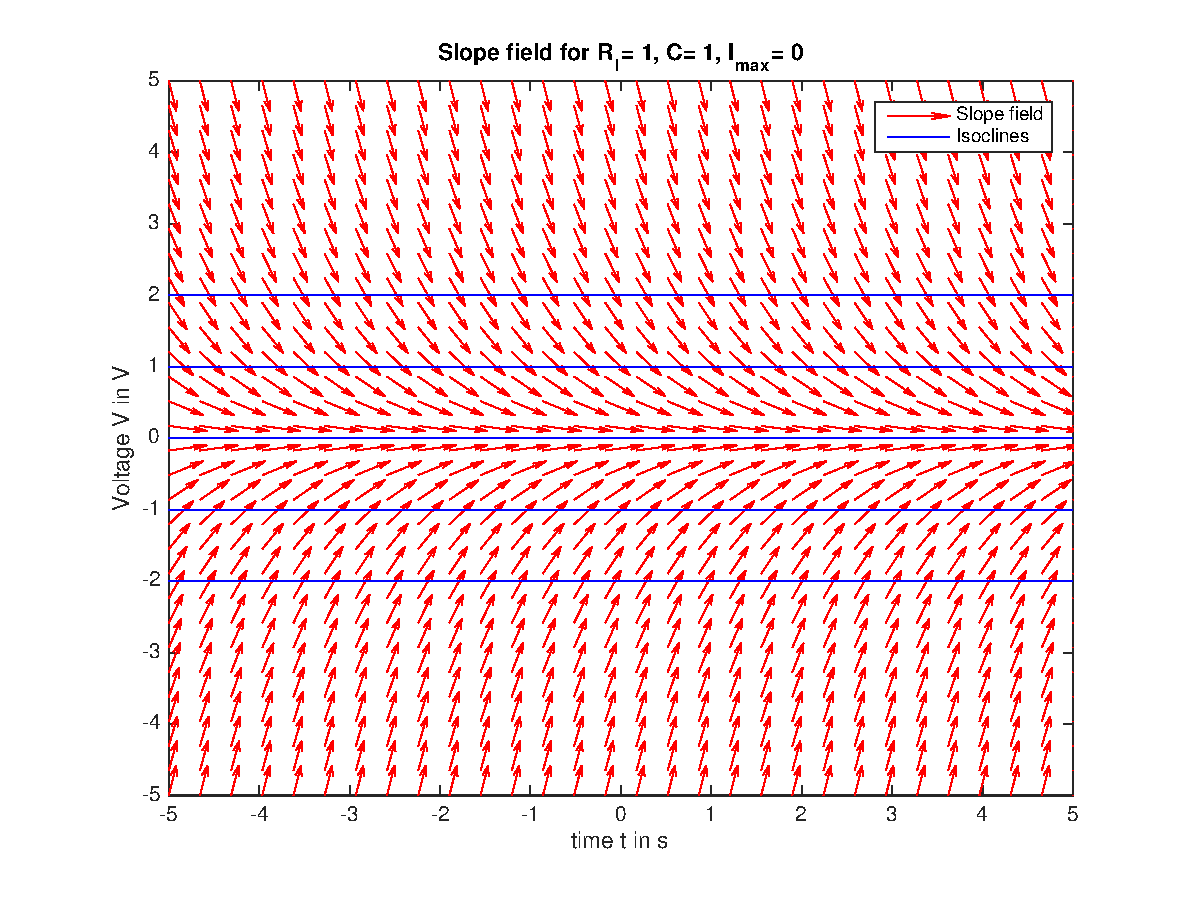
\includegraphics[width=0.85\linewidth]{Plots/lif_1}
\caption{Slope field and isoclines of \textit{equation 4} for $R_l = 1 \Omega$, $C=1$F, $I_{max}=0$A.}
\label{fig:lif_1}
\end{figure}

\begin{figure}[h]
	\centering
	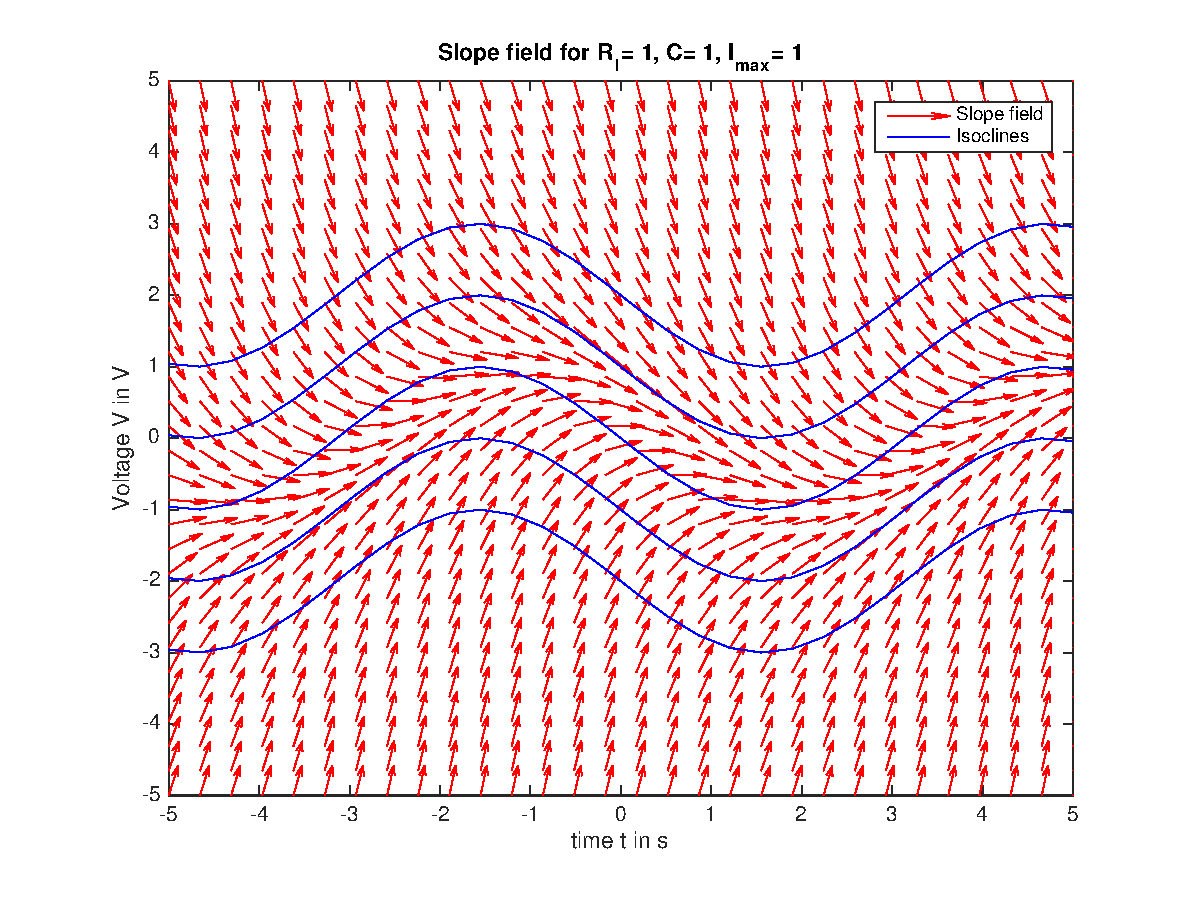
\includegraphics[width=0.85\linewidth]{Plots/lif_2}
	\caption{Slope field and isoclines of \textit{equation 4} for  $R_l = 1 \Omega$, $C=1$F, $I_{max}=1$A.}
	\label{fig:lif_2}
\end{figure}

\clearpage
Now, we add another constant $D = 2$A to the differential equation. As the unit of $D$ is \textit{Ampere}, we will add this constant to the current $I_{ex}$. Equation 4 now looks as following:
\begin{align}
\Rightarrow \frac{du}{dt} &= -\frac{1}{C}\left(\frac{u}{R_l} + I_{max}\cdot sin(t) + D \right) 
\end{align}
This results in the following slope fields and theirs corresponding isoclines:
\begin{figure}[h]
	\centering
	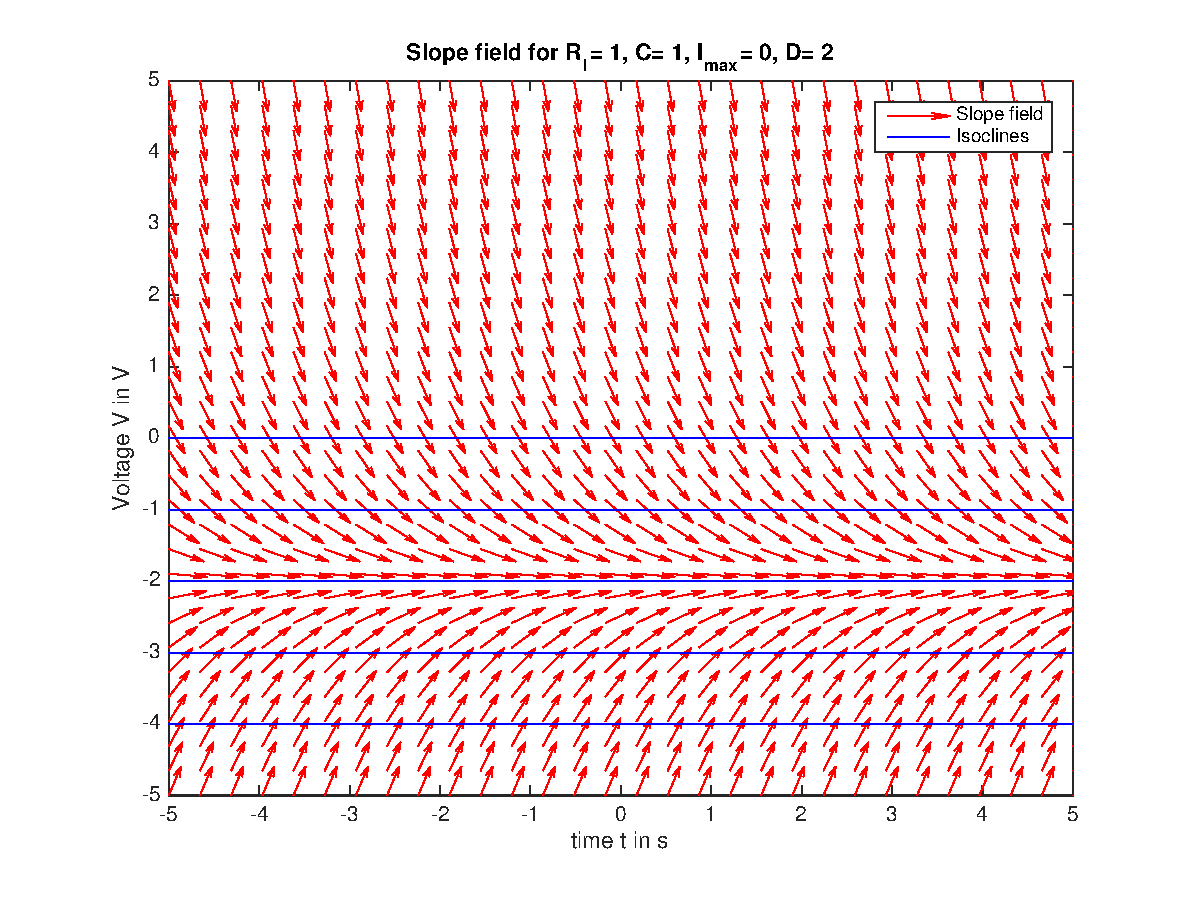
\includegraphics[width=0.85\linewidth]{Plots/lif_3}
	\caption{Slope field and isoclines of \textit{equation 5} for  $R_l = 1 \Omega$, $C=1$F, $I_{max}=0$A and $D=2$A.}
	\label{fig:lif_3}
\end{figure}

\begin{figure}[h]
	\centering
	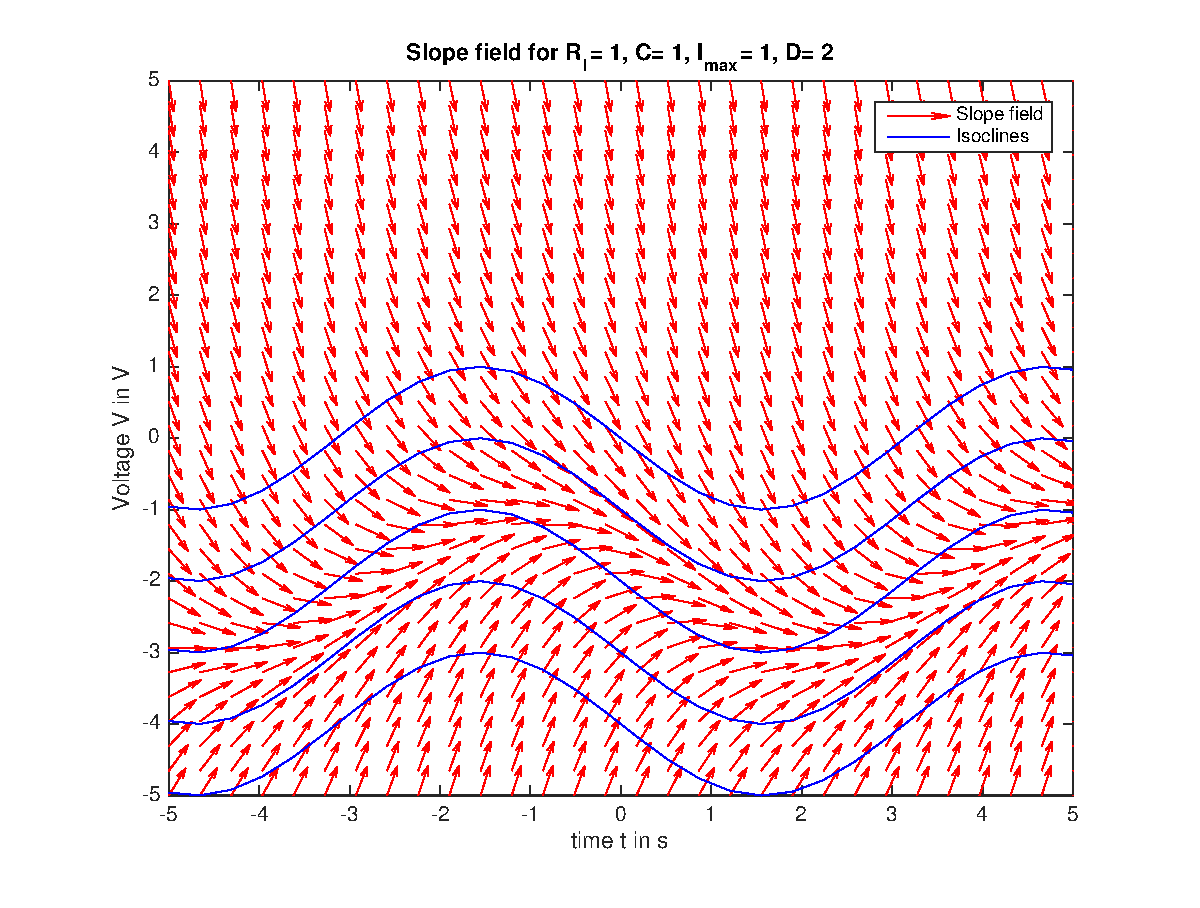
\includegraphics[width=0.85\linewidth]{Plots/lif_4}
	\caption{Slope field and isoclines of \textit{equation 5} for  $R_l = 1 \Omega$, $C=1$F, $I_{max}=1$A and $D=2$A.}
	\label{fig:lif_4}
\end{figure}

\end{document}